\Chapter{Decoder}

\Section{5 lines to 32 lines Decoder}

\begin{tabularx}{\textwidth}{Xp{1cm}X}
   \begin{tabular}{lll}
      Input	        & : $5$	& $\to \ E,D,C,B,A$\\
      Output        & : $32$	& $\to \ O_0 - O_{31}$\\
      Number of ICs & : $\frac{32}{8}=4$ & $\to \ I_0 - I_3$
   \end{tabular}
   &&
   \begin{tabular}{|c|c|l|}\hline
      $E$ & $D$ & Active IC \\\hline
      0 & 0 & $IC_0$ \\\hline
      0 & 1 & $IC_1$ \\\hline
      1 & 0 & $IC_2$ \\\hline
      1 & 1 & $IC_3$ \\\hline
   \end{tabular}
\end{tabularx}

\Heading{Operations:}
   If \ $E=0$ and $D=0$, \ then $IC_0$ is active and other are inactive.\\
   If \ $E=0$ and $D=1$, \ then $IC_1$ is active and other are inactive.\\
   If \ $E=1$ and $D=0$, \ then $IC_2$ is active and other are inactive.\\
   If \ $E=1$ and $D=1$, \ then $IC_3$ is active and other are inactive.

\vspace{3em}
\begin{figure}[h]
   \centering
   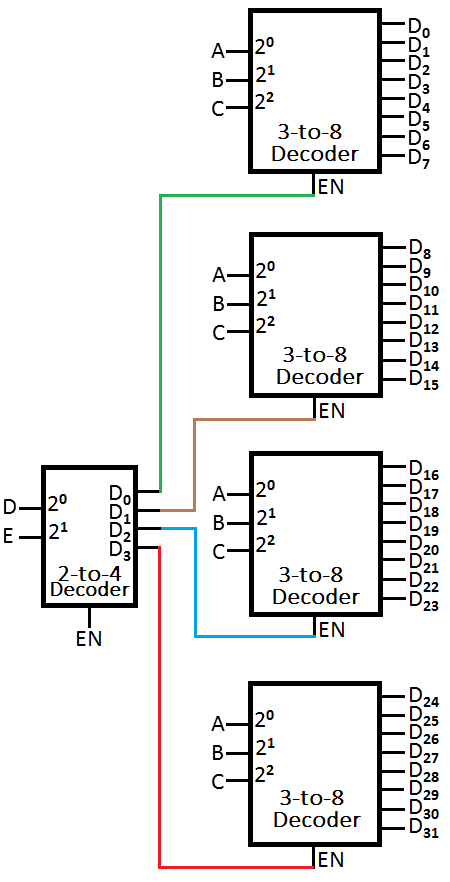
\includegraphics[width=0.35\textwidth]{figures/Decoder_5to32.png}
   \caption{5 lines to 32 lines Decoder using IC-74138}
\end{figure}